\documentclass{article}
\usepackage[utf8]{inputenc}
\usepackage[a4paper, total={6in, 8in}]{geometry}
\usepackage{indentfirst}
\usepackage{authblk}
\usepackage{graphicx}
\usepackage{hyperref}

%\usepackage[square,numbers]{natbib}
%\usepackage[square,sort,comma,numbers]{natbib}
\usepackage[style=numeric]{biblatex}
\addbibresource{references.bib}
\usepackage[dvipsnames]{xcolor}

\usepackage{amsmath}
\usepackage{amsthm} % proof environment
%\usepackage[thref,leref]{ntheorem}
\usepackage{amsfonts}

\usepackage{caption}
\usepackage[shortlabels]{enumitem}
\usepackage{float}
\usepackage{listings}
\usepackage{soul} % highlighting

\newcommand{\floor}[1]{\left\lfloor #1 \right\rfloor}
\newcommand{\ceil}[1]{\left\lceil #1 \right\rceil}

\hypersetup{
  colorlinks=true,
  linkcolor=blue,
  filecolor=blue,
  urlcolor=blue,
  citecolor=OliveGreen
}
\urlstyle{same}

\setlength{\parindent}{2em}
\setlength{\parskip}{1ex}

 \captionsetup[figure]{labelfont={bf},name={Fig.},labelsep=period}
 
 \numberwithin{figure}{section}

\title{\huge{\textbf{A Proof-of-Stake scheme for confidential transactions with hidden amounts}}}
\author{\large{sowle}}
\affil{\small{Zano project \\ \texttt{val@zano.org} \\ \url{https://zano.org}}}
\date{\small{July 2021\footnote{Version 3.0. Last update: 2021-08-08. Check \href{https://github.com/hyle-team/docs/tree/master/PoS/PoS_with_HA}{here} for the latest version.}}}


\begin{document}

\maketitle

\begin{abstract}
This article explores a way of implementing a Proof-of-Stake mining algorithm in an environment where amounts are hidden with homomorphic commitments.

We propose an algorithm which is compatible with such transactions, including transactions with mixed-in decoys.
\end{abstract}

\section{Notation}
Let $\mathbb{G}$ denote the main subgroup of the Ed25519 curve (\cite{ed25519_site}) and $\mathbb{Z}_p$ denote a ring of integers modulo $p$.

$l$ is the order of $\mathbb{G}$: $\#\mathbb{G} = l = 2^{252} + 27742317777372353535851937790883648493$.

For  any  set $X$, $x \stackrel{\$}{\leftarrow} X$ means uniform  sampling of $x$ at random from $X$. 



\section{PoS scheme using open amounts} \label{sec_open_amounts}

\begin{figure}[ht!]
\centering
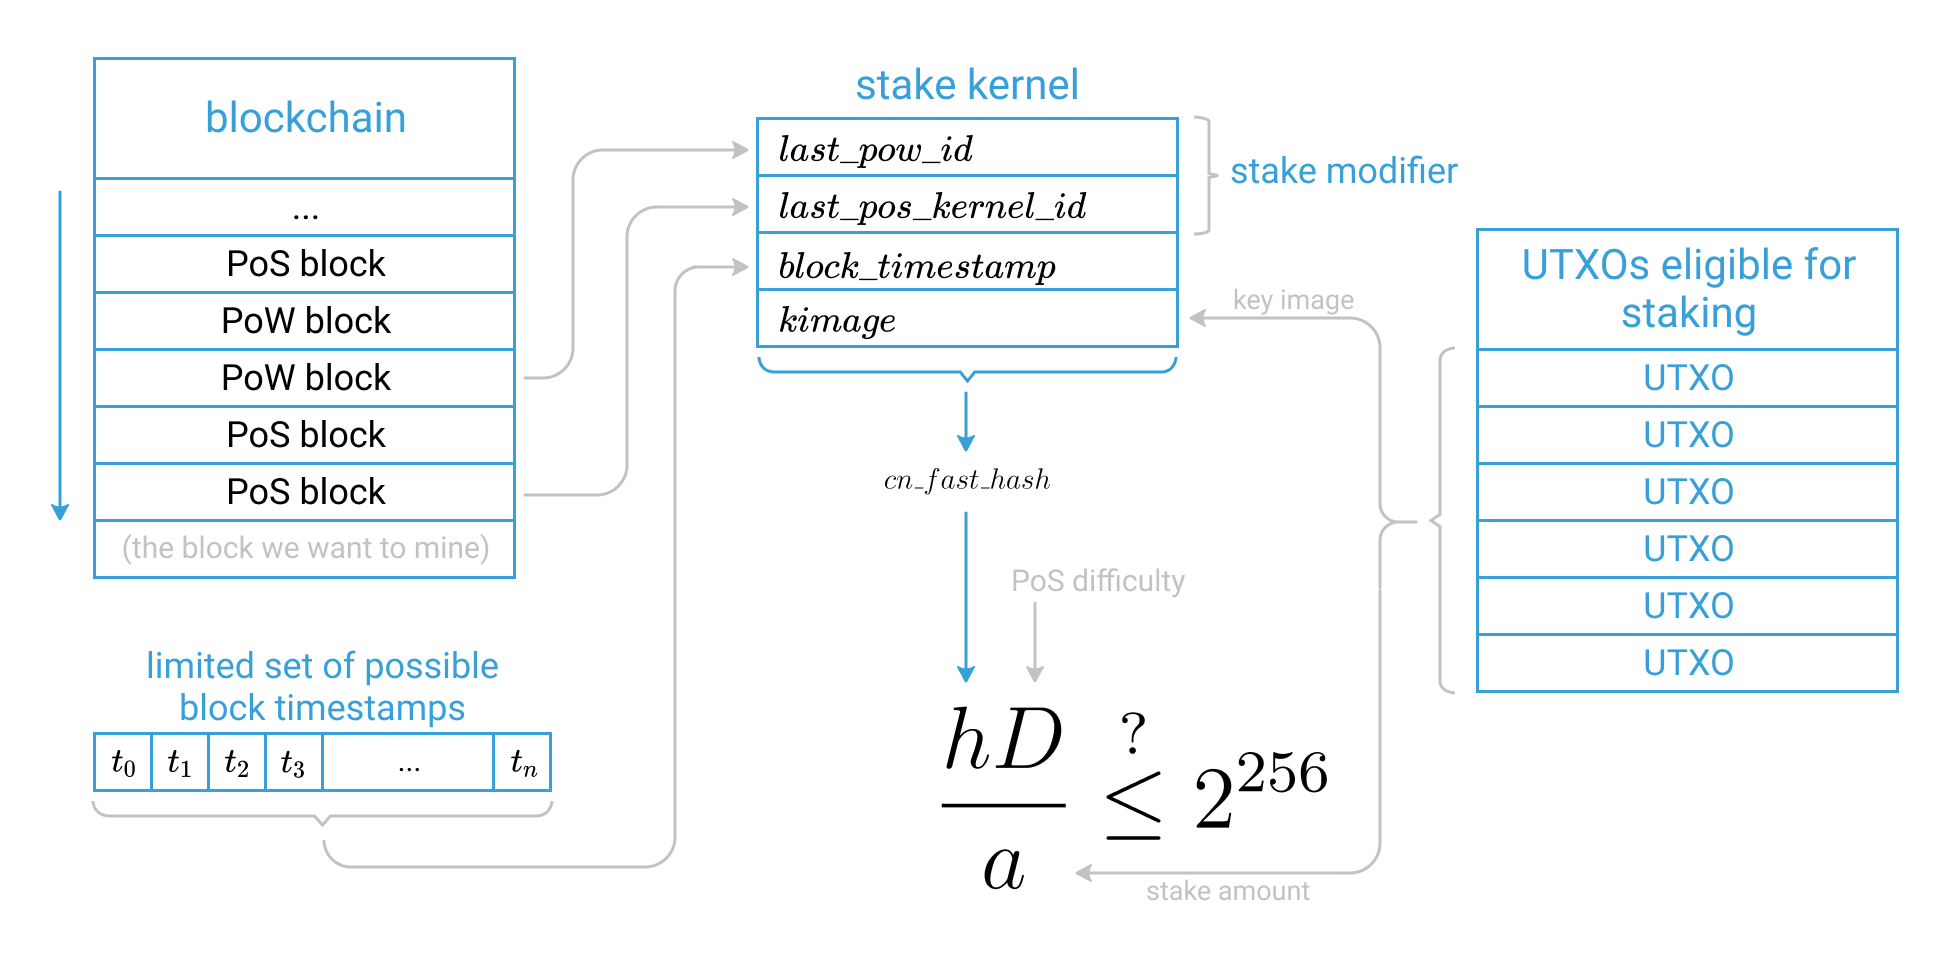
\includegraphics[scale=0.665]{fig_1.png}
\caption{Scheme of the original PoS mining process, as originally implemented in Zano}
\label{fig:1.1}
\end{figure}

\indent
In this section we describe how PoS mining was originally implemented in Zano.

\indent
Suppose Alice has some unspent outputs and wants to mine a PoS block using one of them as a stake. In such a scenario she acts as follows (Fig. \ref{fig:1.1}):

\begin{enumerate}
\item Gets the hash identifier of the last PoW block in the blockchain, $last\_pow\_id$.

\item Gets the last PoS block in the blockchain and gets the stake kernel hash identifier from it, $last\_pos\_kernel\_id$. Together with $last\_pow\_id$ they are called the "stake modifier". It changes each time a new block is added to the blockchain. 

\item Makes set $T$ of all possible timestamps for the new PoS block:
\[ T = \{t : t_{min} \leq t \leq t_{max}, \; t \equiv 0 \mod{15} \} \]
where $t_{min}$ and $t_{max}$ are bound to the current blockchain conditions. For the sake of simplicity we can assume that
\[ t_{min} = \tau - T, \; t_{max} = \tau + T \]
where $T$ is a constant and $\tau$ is the current timestamp established in such a way, that it is the same across all the network nodes.

\item Makes set $U$ of all her unspent transaction outputs (UTXO) that are eligible for staking (i.e. not locked, mature enough etc.). For each output $u$ from $U$ she also precalculates the key image $I_u$.

\item Each pair $(t, u) \in T \times U$ is checked against the PoS winning condition as follows:

    \begin{enumerate}
    \item for output $u$ build \textit{stake kernel} $K_u$ as a concatenation:

    \[ K_u = last\_pow\_id \;\|\; last\_pos\_kernel\_id \;\|\; t \;\|\; I_u \]
    where $I_u$ is the key image of the stake output $u$;
    
    \item Calculate hash $h_u = H_s(K_u)$;
    
    \item Finally, check the main condition:
    \begin{equation} \label{old_pos_main_cond}
    h_u \frac{D}{v_u} \stackrel{?}{\leq} 2^{256} \end{equation} 
    where $D$ is the current PoS difficulty, and $v_u$ is the amount of the stake output $u$. 
    
    \end{enumerate}
    
    If inequality (\ref{old_pos_main_cond}) holds then it means the success of PoS mining! A block with timestamp $t$ and stake input, spending output $u$, can be constructed and broadcast to the network.
    
\end{enumerate}

If for all pairs $(t, u)$ the (\ref{old_pos_main_cond}) does not hold, Alice needs to wait until one of the following happens:
\begin{itemize}
    \item a new block is added to the blockchain (this will change either $last\_pow\_id$ or $last\_pos\_kernel\_id$);
    \item some time passes (this will change $t_{min}$ and $t_{max}$).
\end{itemize}

\indent
Once this happens, Alice can perform another attempt at mining (items 1-5) as all $K_u$, and thus $h_u$, will have different values, giving new opportunities to meet the main condition.


We'd like to note the following important property of (\ref{old_pos_main_cond}): as $h_u$ is the result of cryptographic hash function $H_s$ and could be considered as distributed evenly on $(0..L)$, the probability of meeting the main condition is proportional to output amount $v_u$. 

%\newpage

\section{PoS direct spending scheme using hidden amounts} \label{sec_direct_spend}

\noindent (\textit{Note: this variant of the scheme requires stake inputs to directly refer to their outputs, i.e. without decoys.})

Consider a hidden amount scheme, where amount $v$ of an output is hidden using Pedersen\footcite[More information in original paper by T.P. Pedersen: ][]{Ped} commitment $A$:

\[ A = v G + f H \quad (v < 2^{64}, \; f \neq 0) \]

where $G$ and $H$ are generators for which DL relation is unknown, and $f$ is a random hiding mask.

It's easy to see that (\ref{old_pos_main_cond}) can't be used anymore because it requires using non-hidden $v$. Let's see how the main inequality could be modified.

Suppose Alice has already prepared sets of timestamps ($T$) and outputs ($U$) eligible for staking as mentioned in section \ref{sec_open_amounts}. She then considers each pair $(t, u) \in T \times U$ against the PoS winning condition. She calculates

\[ h = H_s( last\_pow\_id \;\|\; last\_pos\_kernel\_id \;\|\; t \;\|\; I_u ) \]

As we mentioned above, $h$ can be considered as uniform randomness distributed evenly over $\mathbb{Z}_l$. Because hiding mask $f \neq 0$ and it is fixed for the selected output $u$, the multiplication $hf \pmod{l}$ can also be considered as uniform randomness over $\mathbb{Z}_l$. \hl{TODO: formal proof may be needed.}

Taking this into account, Alice checks the slightly adjusted main inequality:

\begin{equation} \label{eq_new_ineq_hf}
    hf < \floor{\frac{l}{D}}v \pmod l
\end{equation}

where $l$ is the order of the main subgroup. Here we moved from $2^{256}$ (used originally in (\ref{old_pos_main_cond})) to $l$ as all scalar operations in all the following equations hold modulo $l$ except the division $\floor{\frac{d_0}{D}}$.

Note that as soon as $D > 2^{64}$ and $v < 2^{64}$, the right side of (\ref{eq_new_ineq_hf}) never overlaps the $l$.

Now we transform the inequality to equality:

\begin{equation} \label{eq_main_eq}
    hf = \floor{\frac{d_0}{D}} v - b_v, \quad D \leq d_0 \leq l, \; b_v < 2^{64}
\end{equation}

Once \eqref{eq_new_ineq_hf} holds, Alice needs to calculate $d_0$ and $b_v$ so that \eqref{eq_main_eq} holds. If then she can convince a verifier of knowing $d_0$, $b_v$ to be in corresponding ranges, she can also convince them that \eqref{eq_new_ineq_hf} holds\footnote{Except with negligible probability in case when $\floor{\frac{d_0}{D}}v < b_v$} for particular $h$, and thus, for pair $(u, t)$. Now we construct such a proof in a NIZK-manner.

Rewriting \eqref{eq_main_eq} slightly:

\begin{equation} \label{eq_part_g}
    \eqref{eq_main_eq} \quad \Leftrightarrow \quad hf - dv + b_v = 0, \quad d = \floor{\frac{d_0}{D}}
\end{equation}

Let $b_f = df - hv$. The following equality holds:

\begin{equation} \label{eq_part_h}
    hv - df + b_f = 0
\end{equation}

Use \eqref{eq_part_g} and \eqref{eq_part_h} as scalar parts for scalar multiplication with $G$ and $H$ correspondingly:

\begin{equation} \label{eq_ge}
\eqref{eq_part_g}, \eqref{eq_part_h} \Rightarrow
\left\{ \begin{aligned} 
  h f - d v + b_v &= 0 \quad | \times G \\
  h v - d f + b_f &= 0 \quad | \times H
\end{aligned} \right.
\end{equation}

Considering commitments $A'=fG+vH, \; A=vG+fH, \; B=b_v G + b_f H$, we can rewrite \eqref{eq_ge} in terms of group element operations: 

\begin{equation} 
    hA'-dA+B=\mathbf{0} \label{eq_ge_fin}
\end{equation}

where $\mathbf{0}$ is the identity element of $\mathbb{G}$.


\subsection{$A'$ proof} \label{a_prime_proof}

As part of the whole PoS proof, Alice needs to convince a verifier that $A' = fG + vH$ without revealing $v$ and $f$. As the verifier knows public $A = vG + fH$ we can construct a Schnorr-like proof as follows:

\begin{enumerate}
    \item Alice generates randomnesses $r_0, r_1 \stackrel{\$}{\leftarrow} \mathbb{Z}_l$ 
    
    \item Calculates $R_0 = r_0 (G + H), R_1 = r_1 (G - H)$
    
    \item Calculates non-interactive challenge $c = H_s(R_0, R_1, A', A)$
    
    \item Calculates $y_0 = r_0 + c(v+f), y_1 = r_1 + c(v-f)$
    
    \item Sends $(c, y_0, y_1)$ to the verifier.

    \item Verifier makes sure that
    \[ c \stackrel{?}{=} H_s(y_0(G+H)-c(A+A'), y_1(G-H)-c(A-A'), A', A)\]
    If the above equation holds, the verifier is convinced that $A+A'=k_0(G+H)$ and $A-A'=k_1(G-H)$ for some $k_0$ and $k_1$, and thus due to Lemma \ref{l_AA'} he is convinced that  $A' = fG + vH$.
\end{enumerate}

In appendix \ref{s_A'_proof_intuition} we give an intuition for the fact that this proof does not reveal parts of commitments.

\subsection{PoS proof} \label{ssec_pos_proof}

Let's summarize the whole scheme.

\begin{enumerate}
    \item Alice prepares a set of possible timestamps $T$ and staking outputs $U$.
    
    \item For each pair $(t, u)$ she calculates $h = H_s(\dots)$ and checks it against the winning condition \eqref{eq_new_ineq_hf}.
    
    \item If \eqref{eq_new_ineq_hf} holds, she calculates:
    \[ \begin{split}
    A' &= fG + vH \\
    d &= \floor{\frac{hf}{v}} + 1\\
    b_v &= dv - hf \\
    b_f &= df - hv \\
    B &= b_v G + b_f H
    \end{split}
    \]
    
    \item Generates proof $(c, y_0, y_1)$ for the fact that $A' = fG + vH$ (section \ref{a_prime_proof}).
    
    \item Makes a PoS block with stake output $u$ and timestamp $t$, and adds PoS proof $\sigma$ to the block's data:
    \begin{equation} \label{eq_pos_proof}
    \sigma = \{ d, A', (c, y_0, y_1), B, \mathcal{R}_B \}
    \end{equation}
    where $\mathcal{R}_B$ is a range proof (e.g. Bulletproofs) for the fact that $b_v < 2^{64}$ 
\end{enumerate}

\noindent 
Verifiers on the network check the PoS block as follows:

\begin{enumerate}
    \item $d \leq \floor{\frac{l}{D}}$
    
    \item Check Schnorr-like signature $(c, y_0, y_1)$ for $A'$.
    
    \item Check $hA'-dA+B=\mathbf{0}$
    
    \item Check range proof $\mathcal{R}_B$
\end{enumerate}


\subsection{Limitations} \label{s_limitations}

The proposed scheme works only under the following conditions:
\begin{itemize}
    \item Proof-of-stake difficulty: $D > 2^{64}$
    \item Output's amount: $v < 2^{64}$
    \item Commitment's mask: $f \neq 0$
\end{itemize}

\subsection{Size of PoS proof}

Let's estimate the size of the proof \eqref{eq_pos_proof}.

It has two group elements, four field elements plus the size of the range proof $\mathcal{R}_B$.

In the case of using Bulletproofs+ \cite{BP+} the size of a single proof with $n = 64$ is 

\[2 \cdot \ceil{\log_2(n)} + 3 = 15\]

group elements and 3 field elements.

In total, for the PoS proof we have 17 group elements and 7 field elements. If both field and group elements have a compressed size of 32 bytes, which is the case for Ed25519 used in Zano, then the total size of the proof can be estimated as $17+7=24$ elements or $24 \cdot 32 = 768$ bytes.


\section{Ring-friendly PoS hidden amount scheme}

The solution we proposed in section \ref{sec_direct_spend} can't be used in the case of a CT-like mining transaction with a non-empty decoy set: in such a transaction the stake input would refer to a \textit{set} of outputs and thus a set of \textit{pseudo} output commitments is used instead of a single commitment $A$ in which the input's hidden amount $v$ is committed to. Therefore, verifiers on the network would not be able to check \eqref{eq_ge_fin} as they don't know the particular $A$. 

Here we propose a solution to this problem.


\subsection{Ring-friendly PoS scheme}

Suppose Alice wants to mine a PoS block, and she already went through steps 1-3 above (subsection \ref{ssec_pos_proof}). She calculated such $A', d, B$ that $ hA' - dA + B = \mathbf{0} $ holds.

Then she continues as follows:
\begin{enumerate}
    \setcounter{enumi}{3} 
    \item Randomly selects a set of apparently unspent decoy outputs $\{u_i\}$ from the blockchain and puts her output, which met the PoS main condition \eqref{eq_new_ineq_hf}, at random index $\pi$ of that set. Note that the $i$-th decoy output has its hidden amount committed to in $A_i$ (and $A_\pi$ is the commitment to her own output). Also note that in general Alice doesn't know amounts $v_i$ and masks $f_i$ for the outputs she selected as decoys.
    
    \item For each decoy output $u_i \; (i \neq \pi)$ Alice generates random values $b_{v,i} \stackrel{\$}{\leftarrow} \mathbb{Z}_{2^{64}}$, $b_{f,i} \stackrel{\$}{\leftarrow} \mathbb{Z}_l$ and commitments to them: 
    
    \begin{equation} \label{rfpos_Bi}
        B_i = b_{v,i} G + b_{f,i} H
    \end{equation} 
    
    She also calculates complementary commitment $A'$:
    
    \begin{equation} \label{rfpos_Aprimei}
        A'_i = h^{-1}(dA_i - B_i)
    \end{equation}
    
    As before, $B_\pi$ and $A'_\pi$ were calculated earlier and correspond to her own output.
    
    Now, consider the system of equations $hA'_i - dA_i + B_i = \mathbf{0}$ or in other notation:
    
    \begin{equation} \label{rfpos_sys}
    \left\{ \begin{aligned} 
        &h A'_0 &- &d A_0 &+ &B_0 &= \mathbf{0} \\
        &&& \dots &&& \\
        &h A'_\pi &- &d A_\pi &+  &B_\pi &= \mathbf{0} \\
        &&& \dots &&& \\
        &h A'_{n-1} &- &d A_{n-1} &+ &B_{n-1} &= \mathbf{0}
    \end{aligned} \right.
    \end{equation}
    
    Here the $\pi$-th equation holds, because of equivalence to \eqref{eq_ge_fin}, and others hold because of \eqref{rfpos_Bi} and \eqref{rfpos_Aprimei}.
    
    \item Consider a pair of group elements $(A_i+A'_i, A_i-A'_i)$. If $i = \pi$ Alice is able to calculate secrets $k_0$ and $k_1$ so the following holds:
    \begin{equation*}
    \left\{ \begin{aligned} 
        A_i + A'_i &= k_0 (G + H) \\
        A_i - A'_i &= k_1 (G - H)
    \end{aligned} \right.
    \end{equation*}
    Indeed: $k_0 = v + f$, $k_1 = v - f$. For all the others $i \neq \pi$ Alice would not be able to calculate such $k_0, k_1$, unless she selected her own output as a decoy (and thus, she knows the corresponding hidden amount and mask). But in such a case \eqref{rfpos_sys} holds only if she is able to calculate appropriate $d$ and $b_{v,i}$ as well, which is equivalent to satisfying \eqref{eq_new_ineq_hf} for that "decoy" output.
    
    According to Lemma \ref{l_AA'}, a proof of knowing $k_0, k_1$ is equivalent to proof that $A'_i = fG + vH$.
    
    Alice adds proof of knowing secret keys $k_0, k_1$ into the main ring signature as two additional layers \footcite[Here we're using terminology and ideas from Multi-layered Linkable Spontaneous Anonymous Group signature proposed in][]{MRL0005}, in order to convince verifiers that $A'_i = fG + vH$ and $A_i = vG + fH$ both hold for the output being spent.
    
    To achieve this, we can extend the main ring signature by adding two more group elements to the calculation of the non-interactive challenge as follows:
    
    \begin{equation*} \begin{aligned}
        c_{\pi+1} &= H_s(\dots, \; \alpha_0 (G + H), \; \alpha_1 (G - H) \\
        c_{i+1} &= H_s(\dots, \; r^0_i (G + H) + c_i (A_i + A'_i), \; r^1_i (G - H) + c_i (A_i - A'_i) \\
        r^0_\pi &= \alpha_0 - c_\pi k_0 \\
        r^1_\pi &= \alpha_1 - c_\pi k_1
     \end{aligned} \end{equation*}
     
     \item Finally, Alice adds PoS signature $\sigma = \{ d, \{A'_i\}, \{B_i\}, \{\mathcal{R}_B_i\} \}$ to the mining transaction, where $\{\mathcal{R}_B_i\}$ are range proofs (e.g. Bulletproofs+) for the fact that $b_{v,i} < 2^{64}$.
\end{enumerate}


\subsection{Verification of ring-friendly PoS scheme} \label{s_verification_ring_friendly}
Verifiers on the network check the PoS block as follows:

\begin{enumerate}
    \item $d \leq \floor{\frac{l}{D}}$
    
    \item Calculate $h$ and check $h A'_i - d A_i + B_i = \mathbf{0}$
    
    \item Check stake input's ring signature with additional layers for $A'_i$
    
    \item Check range proofs $\mathcal{R}_B_i$
\end{enumerate}


\subsection{Size of ring-friendly PoS proof}

Let's estimate the size of the proof for $n-1$ decoy outputs, where the total size of the ring is $n$. Assume we're using aggregated Bulletproofs+ for range proofing. According to \cite{BP+} it comprises $2 \cdot \ceil{\log_2(m) + \log_2(n)} + 3$ elements in $\mathbb{G}$ and 3 elements in $\mathbb{Z}_l$, where $m = 64$ for range $2^{64}$.

For each ring member we need to store 2 elements in $\mathbb{G}$ ($A'_i$ and $B_i$) and, supposedly, only 2 elements in $\mathbb{Z}_l$ for ring signature extension ($r^0_i$ and $r^1_i$).

Additionally, we need to store one element in $\mathbb{Z}_l$ per PoS signature ($d$).

In total we have $2n + 2 \cdot \ceil{\log_2(n)} + 15$ group elements and $2n + 4$ field elements. If both field and group elements have a compressed size of 32 bytes, which is the case for Ed25519 used in Zano, then the total size of additional PoS data can be estimated as $4n + 2 \cdot \ceil{\log_2(n)} + 19$ elements or $128n + 64 \cdot \ceil{\log_2(n)} + 608$ bytes.

%\bibliographystyle{unsrtnat}
%\bibliography{references}
\printbibliography


\newpage
\appendix
\section{Lemmas}

\newtheorem{theorem}{Theorem}%[section]
\newtheorem{corollary}{Corollary}[theorem]
\newtheorem{lemma}[theorem]{Lemma}


\begin{lemma} \label{l_AA'}
Let $v, f \in \mathbb{Z}_l$ and $A = vG + fH$, where $G$ and $H$ -- public generators in cycle group $\mathbb{G}$ of prime order $l$, for both of which DL relation is unknown. The Prover knows $v$ and $f$. The Verifier knows only $A$. If the Prover wants to convince the Verifier that the given $A' = fG + vH$ without revealing secrets $v$ and $f$, it is enough to provide a proof to the fact that he knows $y_0$ and $y_1$ such that:
\[ A + A' = y_0 (G+H) \]
\[ A - A' = y_1 (G-H) \]
\end{lemma}

\begin{proof}
Suppose the Verifier is convinced that the Prover knows $y_0$ and $y_1$ such that the equations above hold. Also suppose that, contrary to the lemma's statement, $A' = aG + bH \neq fG + vH$ where $a, b \in \mathbb{Z}_l$.

Substitute equations for $A$ and $A'$:

\begin{equation*}
    \left\{ \begin{aligned} 
        vG + fH + aG + bH = y_0 (G+H) \\
        vG + fH - aG - bH = y_1 (G-H)
    \end{aligned} \right.
\end{equation*}

As DL relation between $G$ and $H$ is unknown, we can split the equations:

\begin{equation*}
    \left\{ \begin{aligned} 
        (v + a) G &= y_0 G \\
        (f + b) H &= y_0 H \\
        (v - a) G &= y_1 G \\
        (f - b) H &= -y_1 H
    \end{aligned} \right.
\end{equation*}

\begin{equation*}
    \Rightarrow
    \left\{ \begin{aligned} 
        v + a &= f + b \\
        v - a &= b - f
    \end{aligned} \right.
\end{equation*}

\begin{equation*}
    \Leftrightarrow
    \left\{ \begin{aligned} 
        2v &= 2b \\
        2a &= 2f
    \end{aligned} \right.
    \Rightarrow A' = aG + bH = fG + vH 
\end{equation*}

This contradiction concludes the proof.

\end{proof}

\newpage
\section{Intuition for $A'$ proof} \label{s_A'_proof_intuition}

Let us give an intuition for the fact that the $A'$ proof given in subsection \ref{a_prime_proof} for the fact that $A' = fG + vH$  does not reveal $vG$, $fH$, $fG$ or $vH$ to the Verifier. \hl{TODO: formal proof may be needed}

The Verifier gets $\{y_0, y_1, c\}$ from the Prover and thus can construct the following system: 
\begin{equation*} %\label{eq_l}
    \left\{ \begin{aligned} 
        A &= vG + fH \\
        A' &= fG + vH \\
        y_0 &= r_0 + c (v + f) \\
        y_1 &= r_1 + c (v - f) \\
        c &= H_s(r_0(G+H), r_1(G-H), A, A')
    \end{aligned} \right.
\end{equation*}
where all the known values are on the left (except the generators). As $c$ is the result of the cryptographic hash function $H_s$ of fixed arguments it can be treated by the Verifier as a known constant, so we'll exclude the equation for $c$.

Let's multiply all terms in equations for $y_0$ and $y_1$ by $G$ and $H$, and make a substitution:

\begin{equation} \label{eq_A_proof_intuition_greek}
    \left\{ \begin{aligned} 
        y_0 G &= r_0 G + \alpha + \gamma \\
        y_0 H &= r_0 H + \delta + \beta \\
        y_1 G &= r_1 G + \alpha - \gamma \\
        y_1 H &= r_1 H + \delta - \beta \\
        cA &= \alpha + \beta \\
        cA' &= \delta + \gamma
    \end{aligned} \right.
\end{equation}
where
\[
\alpha = cvG \quad \beta = cfH \quad \gamma = cfG \quad \delta = cvH
\]
We would like to show that it's impossible for the Verifier to calculate $\alpha, \beta, \gamma, \delta$.

There are six linearly independent equations in \eqref{eq_A_proof_intuition_greek} and also six unknown values: $\alpha, \beta, \gamma, \delta, r_0, r_1$. It looks like \eqref{eq_A_proof_intuition_greek} could be solved.

However, due to discrete logarithm assumption scalar multiplications $r_0 G$, $r_0 H$, $r_1 G$ and $r_1 H$ should be considered as four independent unknowns rather than two $r_0, r_1$. Therefore, there are eight unknowns in \eqref{eq_A_proof_intuition_greek} and it can not be solved.

Note that if we assume that $r_0 = r_1$ or at least $r_0 k = r_1$, where $k \in \mathbb{Z}_l$ is a known value, the number of unknowns would be reduced to six and the system could be solved, so the Verifier could calculate $\alpha, \beta, \gamma, \delta$.

However, the Prover generates $r_0$ and $r_1$ uniformly at random in $\mathbb{Z}_l$.


\newpage
\section{How to ensure $f \neq 0$}

Here we discuss how to ensure that $f \neq 0$ for commitments in case the underlaying transaction protocol does not guarantee that.

In subsection \ref{s_limitations} we mentioned that the proposed PoS scheme works only under certain conditions, and one of them is the commitment mask $f$ must be nonzero for all staking outputs. The reasoning behind that is simple: suppose Alice prepared a UTXO with amount $v$ committed to $A$ with zero mask $f$: $A = vG + 0H = vG$. Such an output can be staked instantly as the winning condition is met regardless of $h$:

\[ hA' - dA + B = \mathbf{0} \quad \eqref{eq_ge_fin} \quad \stackrel{f = 0}{\Longrightarrow} \quad hvH - dvG + B = \mathbf{0} \]

This implies that for \textit{any} given $h$, point $B = (dv)G + (-hv)H$ and scalar $d = 1$ will satisfy all conditions mentioned in subsection \ref{s_verification_ring_friendly}.

Obviously, this can be solved by providing a proof that $f \neq 0$ for each output in the blockchain and forcing all verifiers to validate it. To avoid such undesirable expenses consider the following idea.

Let's require adding $f'H$ to all the commitments $A_i$ before using them in the PoS protocol, where $f'$ is a public constant that is unknown to Alice when she generates hiding mask $f$ for the output.

For instance, $f'$ can be calculated as $f' = H_s(block\_id)$, where $block\_id$ is the hash identifier of the block containing that output.
Consequently, substituting $f+f'$ for $f$ in \eqref{eq_ge} we get:
\begin{equation*}
\left\{ \begin{aligned} 
  h (f + f') - d v + b_v &= 0 \quad | \times G \\
  h v - d (f + f') + b_f &= 0 \quad | \times H
\end{aligned} \right.
\end{equation*}

Now for \eqref{eq_ge_fin} we obtain:
\[ hA' - dA + B + f'(hG - dH) = \mathbf{0} \]

With such a modification Alice won't be able to gain an advantage when choosing $f$.

\end{document}
